\documentclass{article}
\usepackage{lmodern}
\usepackage[T1]{fontenc}
\usepackage{shapepar}
\usepackage{microtype}
\usepackage{lipsum}
\usepackage{pgfplots}
\pgfplotsset{compat=1.9}
\usepackage{tikz}
\usetikzlibrary{calc,fit,intersections,folding}
\usepackage{pstricks-add}
\usetikzlibrary{arrows.meta,angles,arrows,quotes,backgrounds,calc}

\usepackage[left = 5mm, right = 5mm]{geometry}

\newcommand{\clrone}{black}
\newcommand{\clrtwo}{black}
\newcommand{\clrthree}{black}
\newcommand{\circlesize}{1pt}

\begin{document}
\thispagestyle{empty}

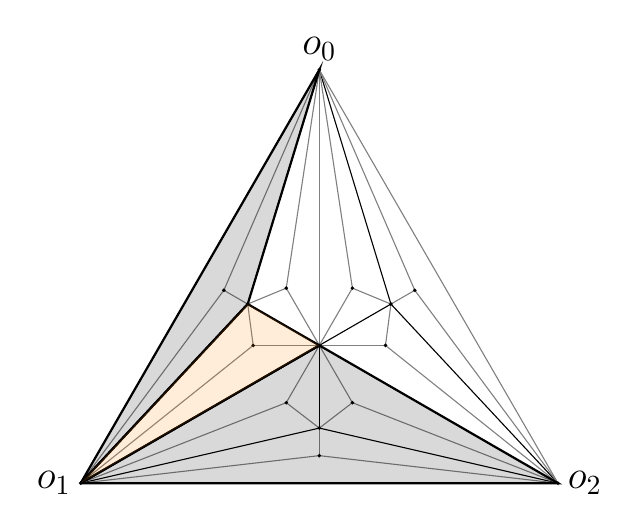
\begin{tikzpicture}[scale = 0.7]

    \coordinate (c) at (0,0);
%outer
    \foreach\a in {0,1,2} {
        \coordinate (o\a) at (90+\a*120:5);
    }
%layer1
    \foreach\a in {0,1,2} {
        \coordinate (1\a) at (30+\a*120:1.5);
    }
%layer2 inner
    \foreach\a in {0,1,2,3,4,5} {
        \coordinate (2i\a) at (\a*60:1.2);
    }
%layer2 outer
    \foreach\a in {0,1,2} {
        \coordinate (2o\a) at (30+\a*120:2);
    }




%%%%        Edges
    \foreach\v/\w in {o0/o1,o1/o2,o2/o0,c/o0,c/o1,c/o2}
    {
        \draw[gray] (\v) -- (\w);
    }
    \foreach\v/\w in {10/o0,10/c,10/o2,11/o0,11/o1,11/c,12/o1,12/c,12/o2}
    {
        \draw (\v) -- (\w);
    }
    \foreach\v/\w in {2i0/c,2i0/10,2i0/o2,2i1/c,2i1/10,2i1/o0,2i2/c,2i2/o0,2i2/11,2i3/c,2i3/11,2i3/o1,2i4/c,2i4/o1,2i4/12,2i5/c,2i5/12,2i5/o2,2o0/10,2o0/o0,2o0/o2,2o1/11,2o1/o0,2o1/o1,2o2/12,2o2/o1,2o2/o2}
    {
        \draw[gray] (\v) -- (\w);
    }

%%%%        Vertices
    \fill (c) circle (\circlesize);
%outer
    \foreach\a in {0,1,2} {
        \fill (o\a) circle (\circlesize);
    }
%layer1
    \foreach\a in {0,1,2} {
        \fill[\clrone] (1\a) circle (\circlesize);
    }
%layer2 inner
    \foreach\a in {0,1,2,3,4,5} {
        \fill[\clrtwo] (2i\a) circle (\circlesize);
    }
%layer2 outer
    \foreach\a in {0,1,2} {
        \fill[\clrtwo] (2o\a) circle (\circlesize);
    }

%%%%        Labels
    \node at (o0) [above] {\Large $o_0$};
    \node at (o1) [left] {\Large $o_1$};
    \node at (o2) [right] {\Large $o_2$};

    \draw[thick] (o1) -- (o0) -- (11) -- (o1);
    \draw[thick] (o1) -- (11) -- (c) -- (o1);
    \draw[thick] (o1) -- (c) -- (o2) -- (o1);

    \fill[opacity = 0.15] (o1) -- (o0) -- (11) -- (o1);
    \fill[opacity = 0.15,orange] (o1) -- (11) -- (c) -- (o1);
    \fill[opacity = 0.15] (o1) -- (c) -- (o2) -- (o1);
\end{tikzpicture}   

\end{document}